\appendix
\section{Minimal-RL Training Details}
\label{app: minimal_rl_training_details}
We mainly follow the Minimal-RL recipe~\citep{xiong2025minimalist} in our experiments to ensure a fair comparison among different rollout sampling strategies. Specifically, we set a series of hyperparameters as in \cref{tab: hyperparameter}:

\begin{table}[h!]
\centering
% \resizebox{\textwidth}{!}{%
\begin{tabular}{@{}cc@{}}
\toprule
Hyperparameter                                 & Value(s)        \\ 
\midrule
\multicolumn{1}{c}{Training Batch Size}      & \multicolumn{1}{c}{1024} \\ 
\multicolumn{1}{c}{Max Prompt Length}        & \multicolumn{1}{c}{1024} \\ 
\multicolumn{1}{c}{Max Response Length}      & \multicolumn{1}{c}{3072} \\ 
\multicolumn{1}{c}{Mini Batch Size}          & \multicolumn{1}{c}{256}  \\ 
\multicolumn{1}{c}{Micro Batch Size Per GPU} & \multicolumn{1}{c}{4}    \\ 
\multicolumn{1}{c}{Learning Rate}            & \multicolumn{1}{c}{$10^{-6}$} \\ 
\bottomrule
\end{tabular}%
% }
\caption{Hyperparameter Setup for Running Minimal-RL recipe. }
\label{tab: hyperparameter}
\end{table}

\section{Off-policy Issue and Truncated Importance Sampling Correction}
\label{sec:off-policy}
\subsection{Sampling Techniques Can Introduce Off-Policy Issue}
\label{subsec:temperature-sampling}
One subtle yet troublesome drawback of reinforcement learning with sampling techniques is that it simultaneously introduces the \emph{off-policy} problem: there is a gap between the behavior policy (used for sampling) and the target policy (being optimized and parametrized by $\theta$). This might introduce instability to the training and cause it to fail (See example training of RLVR with EAD \cref{fig:optim_failure_for_as_offpolicy}).

\begin{figure}[h!]
    \centering
    \begin{subfigure}[b]{0.26\textwidth}
    \centering
    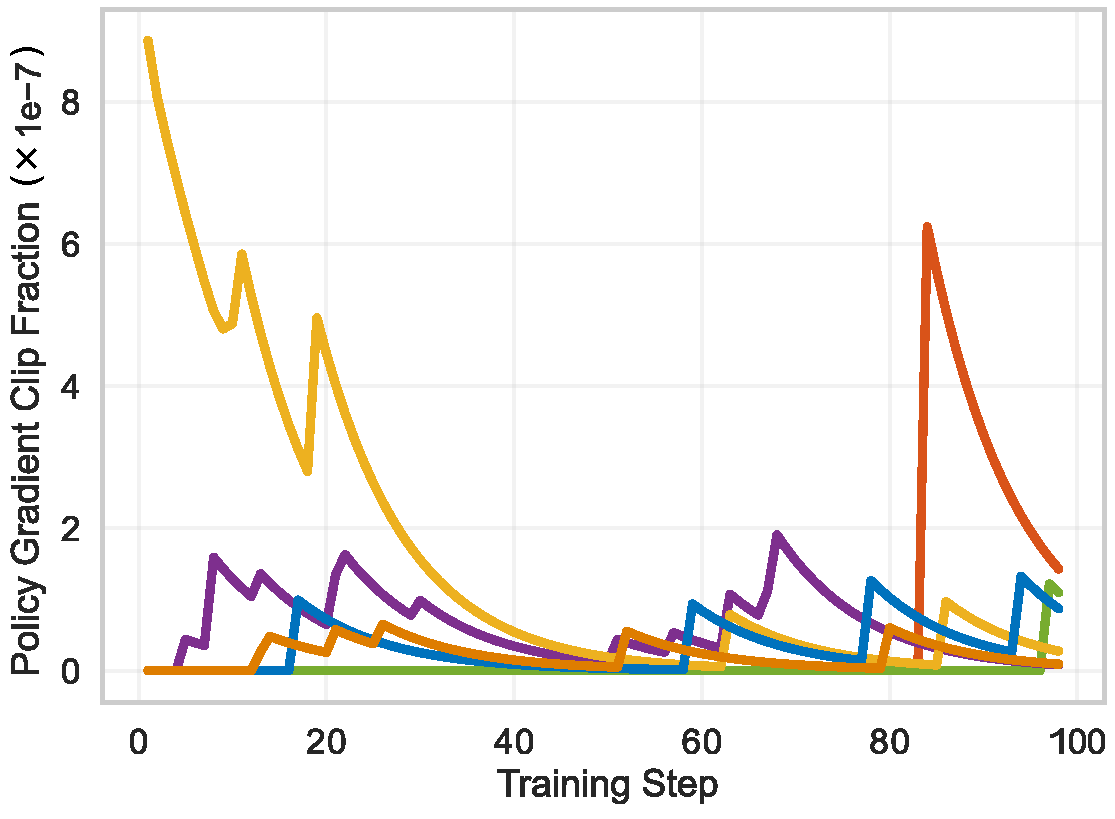
\includegraphics[width=\linewidth]{iclr2026/figures/off_policy_problem/pg_clipfrac_Qwen2.5-Math-1.5B.pdf}
    \caption{Clip Fraction Surge}
    \label{fig: off_policy_pg_clipfrac}
  \end{subfigure}
  \begin{subfigure}[b]{0.28\textwidth}
    \centering
    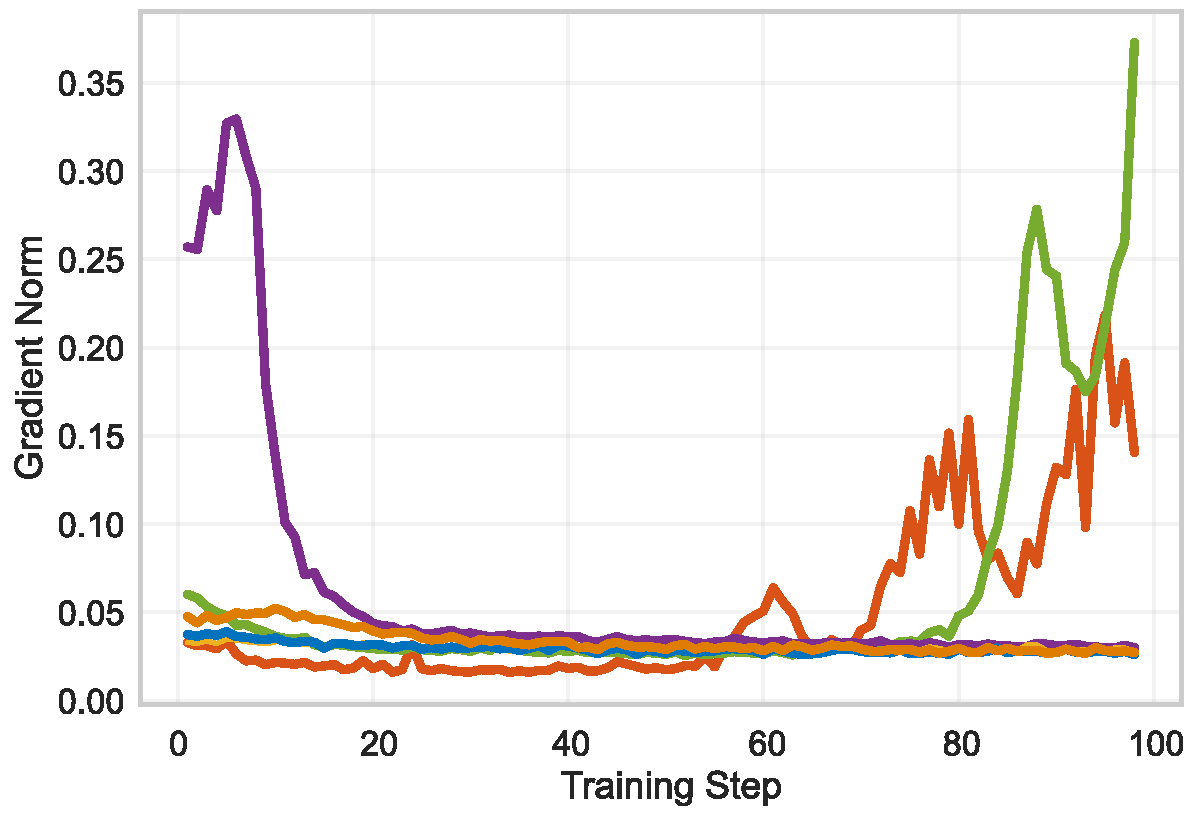
\includegraphics[width=\linewidth]{iclr2026/figures/off_policy_problem/grad_norm_Qwen2.5-Math-1.5B.pdf}
    \caption{Gradient Norm Surge.}
    \label{fig: off_policy_grad_norm}
  \end{subfigure}
   \begin{subfigure}[b]{0.27\textwidth}
    \centering
    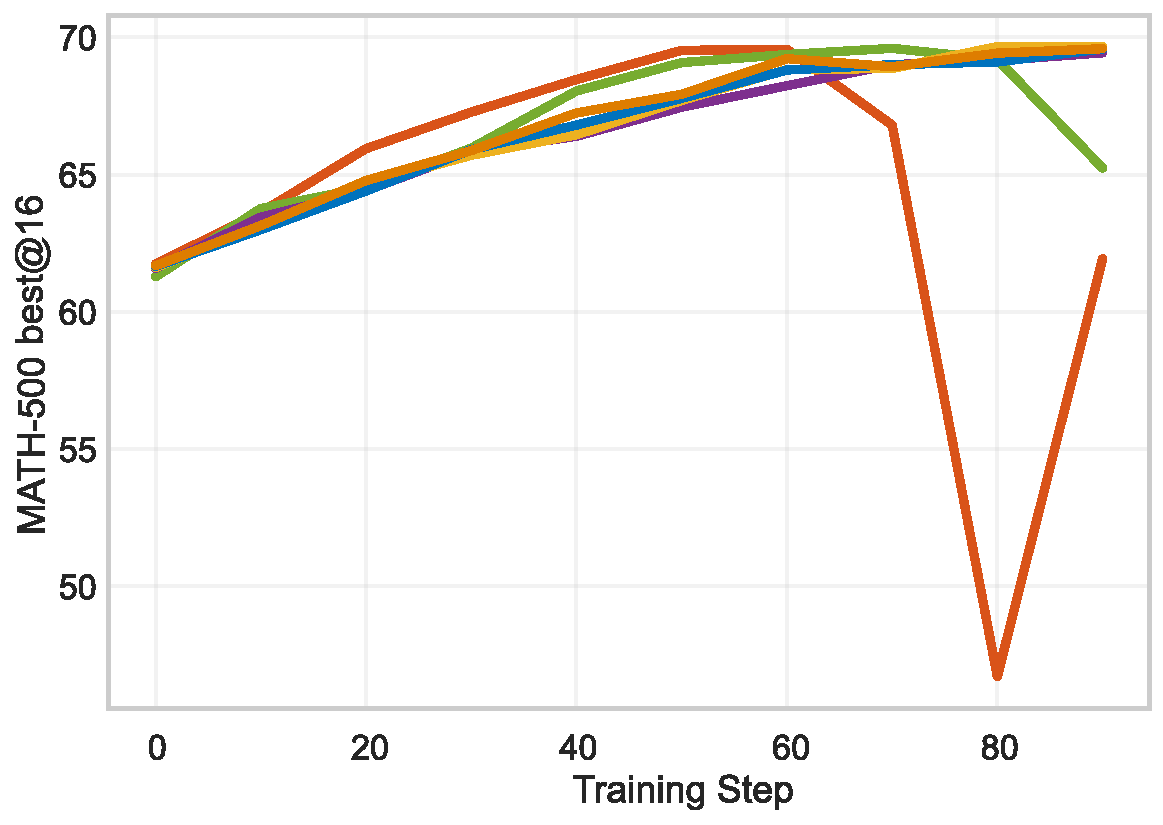
\includegraphics[width=\linewidth]{iclr2026/figures/off_policy_problem/best_at_16_Qwen2.5-Math-1.5B.pdf}
    \caption{Drastic Best@16 Drop}
     \label{fig: off_policy_best_at_16}
  \end{subfigure}
  \begin{subfigure}[t]{0.1\textwidth}
    \centering
    \vspace{-2.5cm}
    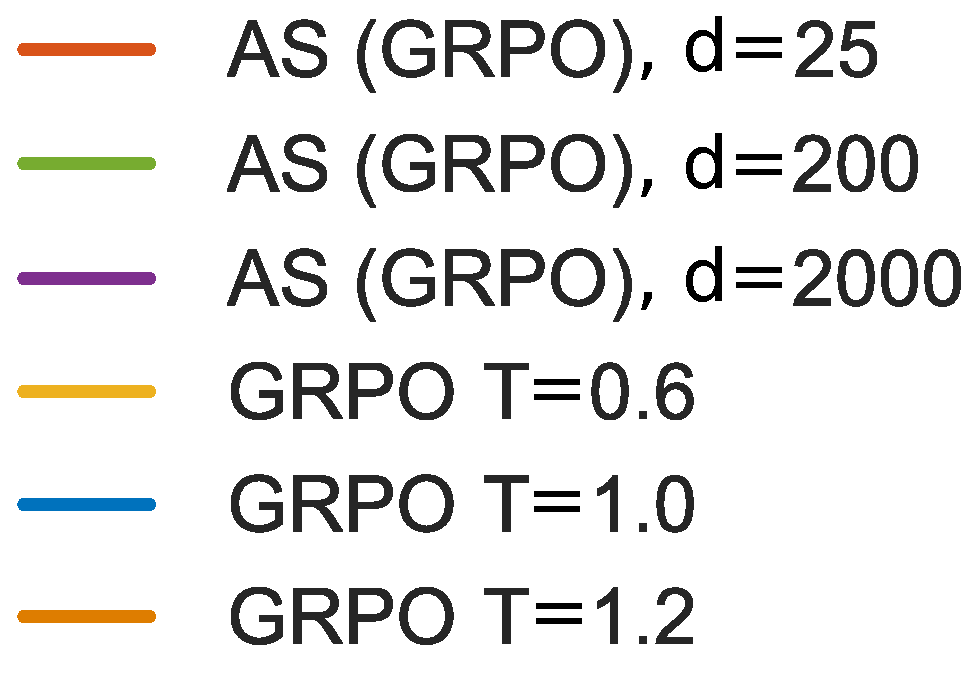
\includegraphics[width=\linewidth]{iclr2026/figures/off_policy_problem/legend-fig3.pdf}
  \end{subfigure}
  \caption{Off-policy samples bring training instability. The base model is Qwen2.5-Math-1.5B.}
  \label{fig:optim_failure_for_as_offpolicy}
\end{figure}

Noted that this off-policy phenomenon widely exists for any efficient sampling framework \citep{yao2025offpolicy} and sampling strategy (for instance, when applying best-of-$n$ sampling \citep{xiong2025minimalist} or filtering out responses \citep{shrivastava2025sample}, the underlying distribution of responses is implicitly altered). To be more precise, we take the policy gradient loss as an example:
\begin{align*}
\E_{x \sim \mathcal{D},y{\sim} \mathbin{\color{red}\pi^{\text{sampling}}_{\theta_{\text{old}}}(\cdot\mid x)}}
\left[\frac{\pi_{\theta}(y\mid x)}{\pi_{\theta_{\text{old}}}(y\mid x)}A(y;x)\right] 
=\E_{x \sim \mathcal{D},y{\sim} \mathbin{\pi_{\theta_{\text{old}}}(\cdot\mid x)}}\left[{\color{red}\frac{\pi^{\text{sampling}}_{\theta_{\text{old}}}(y\mid x)}{\pi_{\theta_{\text{old}}}(y\mid x)}}\times\frac{\pi_{\theta}(y\mid x)}{\pi_{\theta_{\text{old}}}(y\mid x)}A(y;x)\right],
\end{align*}
where $\pi^{\text{sampling}}_{\theta_{\text{old}}}(\cdot\mid x)$ represents the underlying sampling distribution. 
In such case, an extra weight is implicitly added to each response in addition to its advantage $A(y;x)$.

This extra weight can significantly inflate the variance of the policy gradient, posing a stability challenge that our proposed \alg needs to mitigate.
To quantify this effect in our proposed \alg, we now analyze such variance under a standard, fixed \textbf{temperature sampling}.
% This extra weight can significantly inflate the policy gradient's variance, posing a stability challenge that our proposed \alg is designed to mitigate. 
% To motivate the necessity of an annealed schedule, we first quantify the instability introduced by a standard, fixed \textbf{temperature sampling} strategy. This analysis reveals the inherent trade-off between exploration and stability, forming the theoretical basis for our dynamic approach.

% For this technique, the sampling policy is a temperature-annealed version of the target policy, i.e., $\pi^{\text{sampling}}_{\theta_{\text{old}}} = \pi_{\theta_{\text{old}}}(\cdot\mid x;\tau)$, where $\tau$ is the temperature.
% The severity of the resulting off-policy issue can then be precisely measured by the variance of the importance-weighted gradient estimator, which we investigate below.

% \paragraph{Temperature Sampling.} 
We use $\tau=1$ to define a policy $\pi$ and consider the effect of $\tau$ on the variance of the gradient estimator. We reduce the problem to analyzing the variance inflation factor
\begin{equation}
\label{eq:variance-inflation-factor}
\mathbb{E}_{y\sim\pi(\cdot\mid x;\tau)}\left[\frac{\pi(y\mid x;1)^2}{\pi(y\mid x;\tau)^2}\right].
\end{equation}
We begin with one-token case. Let $o_i$ denote the $i$th token in the vocabulary $V$ and $h_i$ is its logit. Then \eqref{eq:variance-inflation-factor} can be rewritten as
\begin{align*}
    \sum_{i=1}^{|V|}\frac{h_i/(\sum_{j=1}^{|V|} h_j)}{h^{1/\tau}_i/(\sum_{j=1}^{|V|} h^{1/\tau}_j)}\times\frac{h_i}{\sum_{j=1}^{|V|} h_j}
    = \frac{\sum_{i=1}^{|V|} h_i^{2-1/\tau}\sum_{i=1}^{|V|} h^{1/\tau}_i}{\left(\sum_{i=1}^{|V|} h_i\right)^2}
\end{align*}

\begin{proposition}
Suppose $h_i\in[0,1]$ for all $i\in V$.
$\sum_{i=1}^{|V|} h_i^{2-1/\tau}\sum_{i=1}^{|V|} h^{1/\tau}_i$ is decreasing when $\tau\le1$ and increasing when $\tau\ge1$, which implies it has a global minimum at $\tau=1$.
\end{proposition}
\begin{proof}
Let $x=1/\tau$. We define 
\[
f(x)=\log\left(\sum_{i=1}^{|V|} h_i^{2-x}\right)+\log\left(\sum_{i=1}^{|V|} h^{x}_i\right).
\]
Its derivative is
\[
f'(x)=\frac{-\sum_{i=1}^{|V|} h_i^{2-x}\log h_i}{\sum_{i=1}^{|V|} h_i^{2-x}}
+\frac{\sum_{i=1}^{|V|} h_i^{x}\log h_i}{\sum_{i=1}^{|V|} h_i^{x}}.
\]
To analyze the sign of $f'(x)$, we define a helper function $g(x) = \frac{\sum_{i=1}^{|V|} h_i^{x}\log h_i}{\sum_{i=1}^{|V|} h_i^{x}}$. Then, $f'(x)=g(x)-g(2-x)$ and its sign depends on whether $g(x)$ is greater than, less than, or equal to $g(2-x)$. We take a look at derivative of $g$:
\[
g'(x) = \frac{\left(\sum_{i=1}^{|V|} h_i^{x}(\log h_i)^2\right) \left(\sum_{i=1}^{|V|} h_i^{x}\right) - \left(\sum_{i=1}^{|V|} h_i^{x}\log h_i\right)^2}{\left(\sum_{i=1}^{|V|} h_i^{x}\right)^2}\ge0.
\]
Hence, $g$ is an increasing function and
\begin{equation*}
\begin{cases}
~f'(x)=g(x)-g(2-x)\ge0,~~\mathrm{when}~x\ge1\\
~f'(x)=g(x)-g(2-x)=0,~~\mathrm{when}~x=1\\
~f'(x)=g(x)-g(2-x)\le0,~~\mathrm{when}~x\le1.
\end{cases}
\end{equation*}
Accordingly, $f$ is increasing when $x\ge1$ and is decreasing when $x\le1$. Then the proposition easily follows.
\end{proof}

The same conclusion can be proved for multiple-token sequence by induction. Therefore, we get that
when the temperature is far from 1, the off-policy issue could be severe and lead to large variance of the gradient estimator. 


\subsection{Truncated Importance Sampling Ratio Correction}
\label{subsec:tis-correction}
% Such techniques can extensively be applied to prevent extreme likelihood ratios and the resulting huge gradients, thereby enhancing training stability. 
To cancel such bias, an importance sampling ratio can be introduced~\citep{hilton2022batch,yao2025offpolicy}:
% Such bias can be corrected by introducing an importance sampling ratio:
\begin{align*}
\E_{x \sim \mathcal{D},y{\sim} \mathbin{\pi_{\theta_{\text{old}}}(\cdot\mid x)}}\left[\frac{\pi_{\theta}(y\mid x)}{\pi_{\theta_{\text{old}}}(y\mid x)}A(y;x)\right]
=
\E_{x \sim \mathcal{D},y{\sim} \mathbin{\color{red}\pi^{\text{sampling}}_{\theta_{\text{old}}}(\cdot\mid x)}}
\left[{\color{red}\frac{\pi_{\theta_{\text{old}}}(y\mid x)}{\pi^{\text{sampling}}_{\theta_{\text{old}}}(y\mid x)}}\times\frac{\pi_{\theta}(y\mid x)}{\pi_{\theta_{\text{old}}}(y\mid x)}A(y;x)\right]. 
\end{align*}
To further prevent negative effects by the extreme likelihood ratios and boost training stability, we truncate the likelihood ratio with an upper bound. That is, \emph{truncated importance sampling} technique \citep{heckman1998matching}. Taking the vanilla policy gradient loss as an example, the modified loss for EAD is as follows:
\begin{equation*}
\label{eq:tis-pg}
\E_{x \sim \mathcal{D},y{\sim}{\pi^{\text{EAD}}_{\theta_{\text{old}}}(\cdot\mid x)}}
\left[{\color{blue}\min\left(\frac{\pi_{\theta_{\text{old}}}(y\mid x)}{\pi^{\text{EAD}}_{\theta_{\text{old}}}(y\mid x)},\varepsilon\right)}\frac{\pi_{\theta}(y\mid x)}{\pi_{\theta_{\text{old}}}(y\mid x)}A(y;x)\right].
\end{equation*}

% One subtle yet troublesome drawback of RLVR with \algname is that it simultaneously introduces the \emph{off-policy} problem, which might cause training to fail (See \cref{fig:optim_failure_for_as_offpolicy}). This issue arises from the mismatch between the distribution generating the responses and the distribution being optimized. 
% To cancel such bias while guarantee training robustness, we add \emph{truncated importance sampling} technique \citep{heckman1998matching}. Taking the vanilla policy gradient loss as an example, the modified loss is as follows:
% \begin{equation}
% \label{eq:tis-pg}
% \E_{x \sim \mathcal{D},y{\sim}{\pi^{\text{EAD}}_{\theta_{\text{old}}}(\cdot\mid x)}}
% \left[{\color{blue}\min\left(\frac{\pi_{\theta_{\text{old}}}(y\mid x)}{\pi^{\text{EAD}}_{\theta_{\text{old}}}(y\mid x)},\varepsilon\right)}\frac{\pi_{\theta}(y\mid x)}{\pi_{\theta_{\text{old}}}(y\mid x)}A(y;x)\right].
% \end{equation}
% In particular, we pre-specify $\varepsilon=2$.


% \section{Higher Temperature Increases Entropy}
% \label{app: temperature_and_entropy}
\newpage
% \section{Additional Experimental Results}
% % \begin{wrapfigure}{r}{0.43\textwidth}
% % \vspace{-0.5in}
% \begin{figure}[h!]
%     \centering
%     
\includegraphics[width=0.75\linewidth]{iclr2026/figures/reverse_annealing/best_at_16_Qwen2.5-Math-1.5B-new.pdf}
%     % \vspace{-0.25in}
%     \caption{Reverse Annealing ablation experiment results. The reverse schedule fails to surpass normal temperature sampling, confirming that an annealing (decreasing) schedule is essential for performance gains.} 
%     \label{fig: reverse_annealing}
%     % \vspace{-0.7in}
% \end{figure}
% % \end{wrapfigure}

% \begin{figure}[ht!]
%      \centering
%      \begin{subfigure}[h]{0.49\textwidth}
%          \centering
%          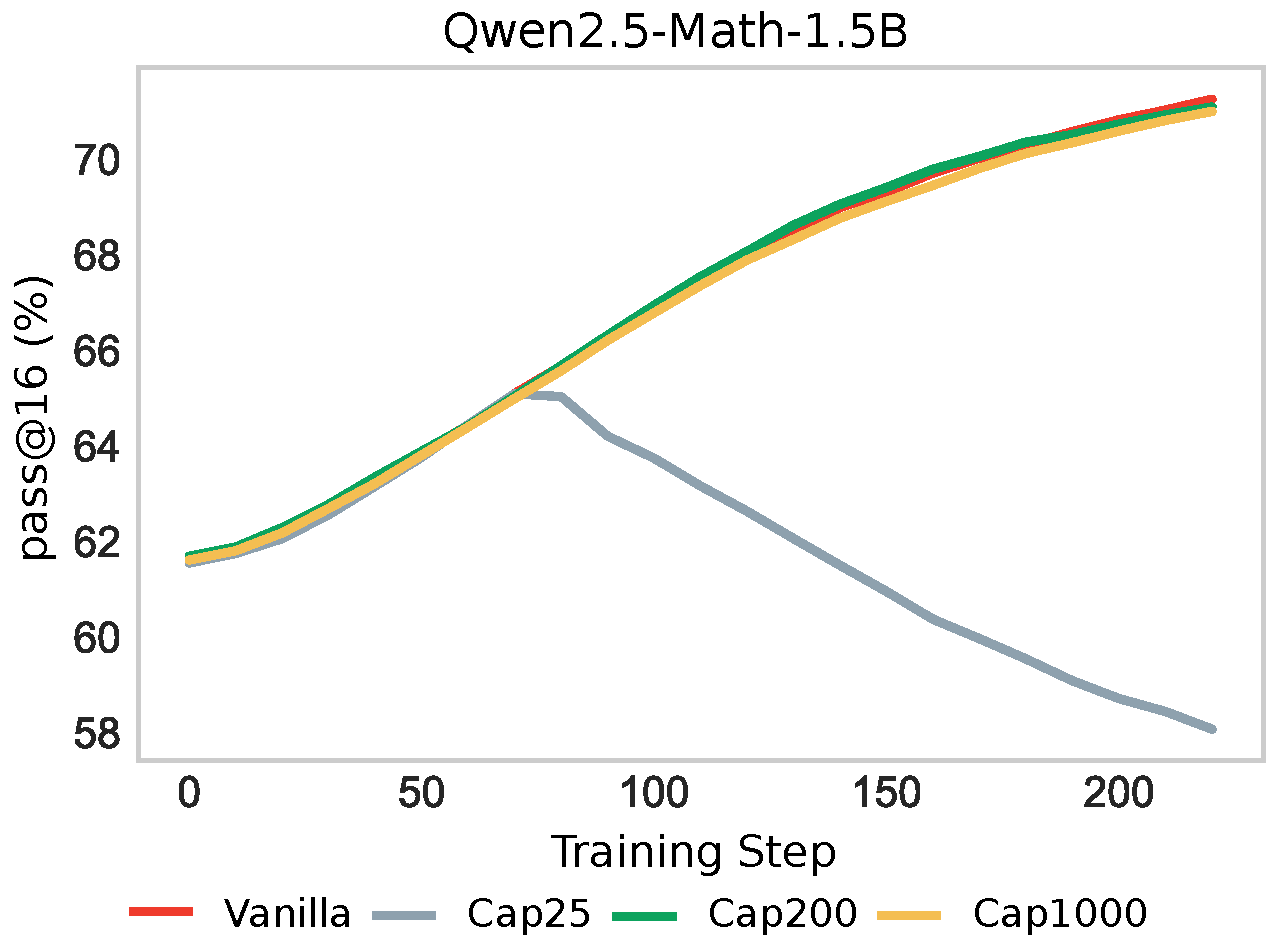
\includegraphics[width=\textwidth]{iclr2026/figures/ablation_cap/best_at_16_Qwen2.5-Math-1.5B-new.pdf}
%          \caption{Decay cap $d_{\max}$.}
%          \label{fig: ablation_cap}
%      \end{subfigure}
%      \begin{subfigure}[h]{0.49\textwidth}
%          \centering
%          
\includegraphics[width=\textwidth]{iclr2026/figures/ablation_growth_factor_and_decay_freq_init/best_at_16_Qwen2.5-Math-1.5B-new.pdf}
%          \caption{Growth factor $\alpha$ and initial decay $d_0$.}
%          \label{fig: ablation_growth_factor_and_decay_freq_init}
%      \end{subfigure}
% \vspace{-0.1in}
% \caption{Ablation on hyperparameter sensitivity. \textbf{Left:} Ablation on decay cap $d_{\max}$. ``Vanilla'' denotes EAD with the default $d_{\max}=40,000$. Setting $d_{\max}=25$ (where $d_0=25$) mimics a fixed temperature schedule (effectively $\alpha=0$), leading to performance drops as the schedule fails to adapt to longer responses. \alg remains robust provided $d_{\max}$ allows for smooth temperature reduction (e.g., $d_{\max} \ge 200$). \textbf{Right:} Ablation on growth factor $\alpha$ and initial decay $d_0$. With a small $d_0$, a positive growth factor ($\alpha > 0$) is required to adapt to increasing response lengths and maintain a smooth intra-sequence schedule. While a large $d_0$ ensures smoothness even with $\alpha=0$, it limits exploration, resulting in lower learning efficiency.}
% \label{fig:hyper-parameter-sensitivity}
% \end{figure}

\newpage
\section{Proof of Temperature-Entropy Relationship}
\label{app:entropy_proof}

% \newtheorem{proposition}{Proposition}
\begin{proposition}
The entropy of the softmax distribution is a non-decreasing function of the temperature $\tau > 0$.
\end{proposition}

\begin{proof}
The strategy is to show that the entropy $H$ is a non-increasing function of the inverse temperature $\beta = 1/\tau > 0$.
The probability of sampling token $v$ with temperature $\tau$ is given by the policy $\pi_\theta$. For simplicity in the derivation, we denote this probability as $p_v(\tau)$:
\[
p_v(\tau) \triangleq \pi_\theta(y_t=v \mid [x, y_{<t}]; \tau)
\]
% = \frac{\exp(h_v / \tau)}{\sum_{v' \in V} \exp(h_{v'} / \tau)}.$

Let $h_v$ be the logit for a token $v$ in the vocabulary $V$. The probability of a token as a function of $\beta$ is given by:
\[
p_v(\beta) = \frac{\exp(\beta h_v)}{\sum_{v' \in V} \exp(\beta h_{v'})} \triangleq \frac{\exp(\beta h_v)}{Z(\beta)},
\]
where $Z(\beta)$ is the partition function. The entropy, as a function of $\beta$, is:
\[
H(\beta) = -\sum_{v \in V} p_v(\beta) \log p_v(\beta).
\]
We can rewrite the entropy by substituting $\log p_v(\beta) = \beta h_v - \log Z(\beta)$:
\begin{align*}
H(\beta) &= -\sum_{v \in V} p_v(\beta) (\beta h_v - \log Z(\beta)) \\
&= \log Z(\beta) \left(\sum_{v \in V} p_v(\beta)\right) - \beta \sum_{v \in V} h_v p_v(\beta) \\
&= \log Z(\beta) - \beta \cdot \mathbb{E}_{v \sim p(\beta)}[h_v].
\end{align*}
Now, we differentiate $H(\beta)$ with respect to $\beta$. Let $\bar{h}(\beta) = \mathbb{E}[h_v]$.
\[
\frac{dH}{d\beta} = \frac{d}{d\beta}(\log Z(\beta)) - \frac{d}{d\beta}(\beta \bar{h}(\beta)).
\]
First, we find the derivative of the log-partition function:
\[
\frac{d}{d\beta}(\log Z(\beta)) = \frac{Z'(\beta)}{Z(\beta)} = \frac{\sum_v h_v \exp(\beta h_v)}{Z(\beta)} = \sum_v h_v p_v(\beta) = \bar{h}(\beta).
\]
Next, we use the product rule for the second term:
\[
\frac{d}{d\beta}(\beta \bar{h}(\beta)) = \bar{h}(\beta) + \beta \frac{d\bar{h}}{d\beta}.
\]
Combining these gives:
\[
\frac{dH}{d\beta} = \bar{h}(\beta) - \left(\bar{h}(\beta) + \beta \frac{d\bar{h}}{d\beta}\right) = -\beta \frac{d\bar{h}}{d\beta}.
\]
The derivative $\frac{d\bar{h}}{d\beta}$ is the variance of the logits. We can show this by differentiating $\bar{h}(\beta)$:
\begin{align*}
\frac{d\bar{h}}{d\beta} &= \frac{d}{d\beta}\left( \frac{\sum_v h_v \exp(\beta h_v)}{Z(\beta)} \right) \\
&= \frac{(\sum_v h_v^2 \exp(\beta h_v))Z(\beta) - (\sum_v h_v \exp(\beta h_v))Z'(\beta)}{Z(\beta)^2} \\
&= \sum_v h_v^2 p_v(\beta) - \left(\sum_v h_v p_v(\beta)\right)\left(\frac{Z'(\beta)}{Z(\beta)}\right) \\
&= \mathbb{E}[h^2] - (\mathbb{E}[h])^2 = \mathrm{Var}_{v \sim p(\beta)}(h_v).
\end{align*}
Substituting this back, we arrive at the final expression for the derivative of entropy:
\[
\frac{dH}{d\beta} = -\beta \cdot \mathrm{Var}_{v \sim p(\beta)}(h_v).
\]
By definition, the temperature $\tau > 0$, so the inverse temperature $\beta > 0$. The variance of any random variable is non-negative. This can be formally shown using \textbf{Jensen's inequality}: for the convex function $\phi(x)=x^2$, we have $\mathbb{E}[\phi(h)] \ge \phi(\mathbb{E}[h])$, which means $\mathbb{E}[h^2] \ge (\mathbb{E}[h])^2$, and thus $\mathrm{Var}(h) \ge 0$.

Therefore, the derivative of entropy with respect to $\beta$ is non-positive:
\[
\frac{dH}{d\beta} = \underbrace{-\beta}_{\le 0} \cdot \underbrace{\mathrm{Var}(h_v)}_{\ge 0} \le 0.
\]
Since $H(\beta)$ is a non-increasing function of $\beta$, and $\beta$ is inversely proportional to $T$, it follows that $H(\tau)$ must be a non-decreasing function of the temperature $\tau$.
\end{proof}

\section{Increasing Length in RL Training}
\label{app: increased_length}
% During RL training, we additionally find that compared with normal temperature sampling, \alg can incentivize the model to generate longer reasoning chains to solve problems, especially for 7B models, as demonstrated in \cref{fig: response_length}. Here, EAD is applied in the DAPO algorithm for sampling rollouts. By manually examine the outputs, we find that at the beginning, the rollout samples produced by both \alg and normal temperature sampling will try to call the Python program to solve the math question, leading to relatively complicated solutions even for simple questions. With the training goes on, the model gradually learns to use pure mathematical way to solve the problem, and the response length decreases. For normal temperature sampling, the response lengths would usually remain stable, but for \alg, it will continue to increase the response length for harder problems and get better performance, leading to the increased response length. 
During RL training, our algorithm (\alg) incentivizes the model to generate longer, more effective reasoning chains for difficult problems, especially for 7B models (\cref{fig: response_length}). While both \alg and temperature sampling initially learn to shorten their responses by shifting from complex code-based solutions to direct mathematical reasoning, their behavior later diverges. The response length from temperature sampling stabilizes, whereas \alg learns to selectively increase reasoning length for harder problems, which boosts final performance. For these experiments, EAD is applied in the DAPO algorithm for sampling rollouts. We use the same training setup as detailed in \cref{sec:experiments}. 

\begin{figure}[h!]
\centering
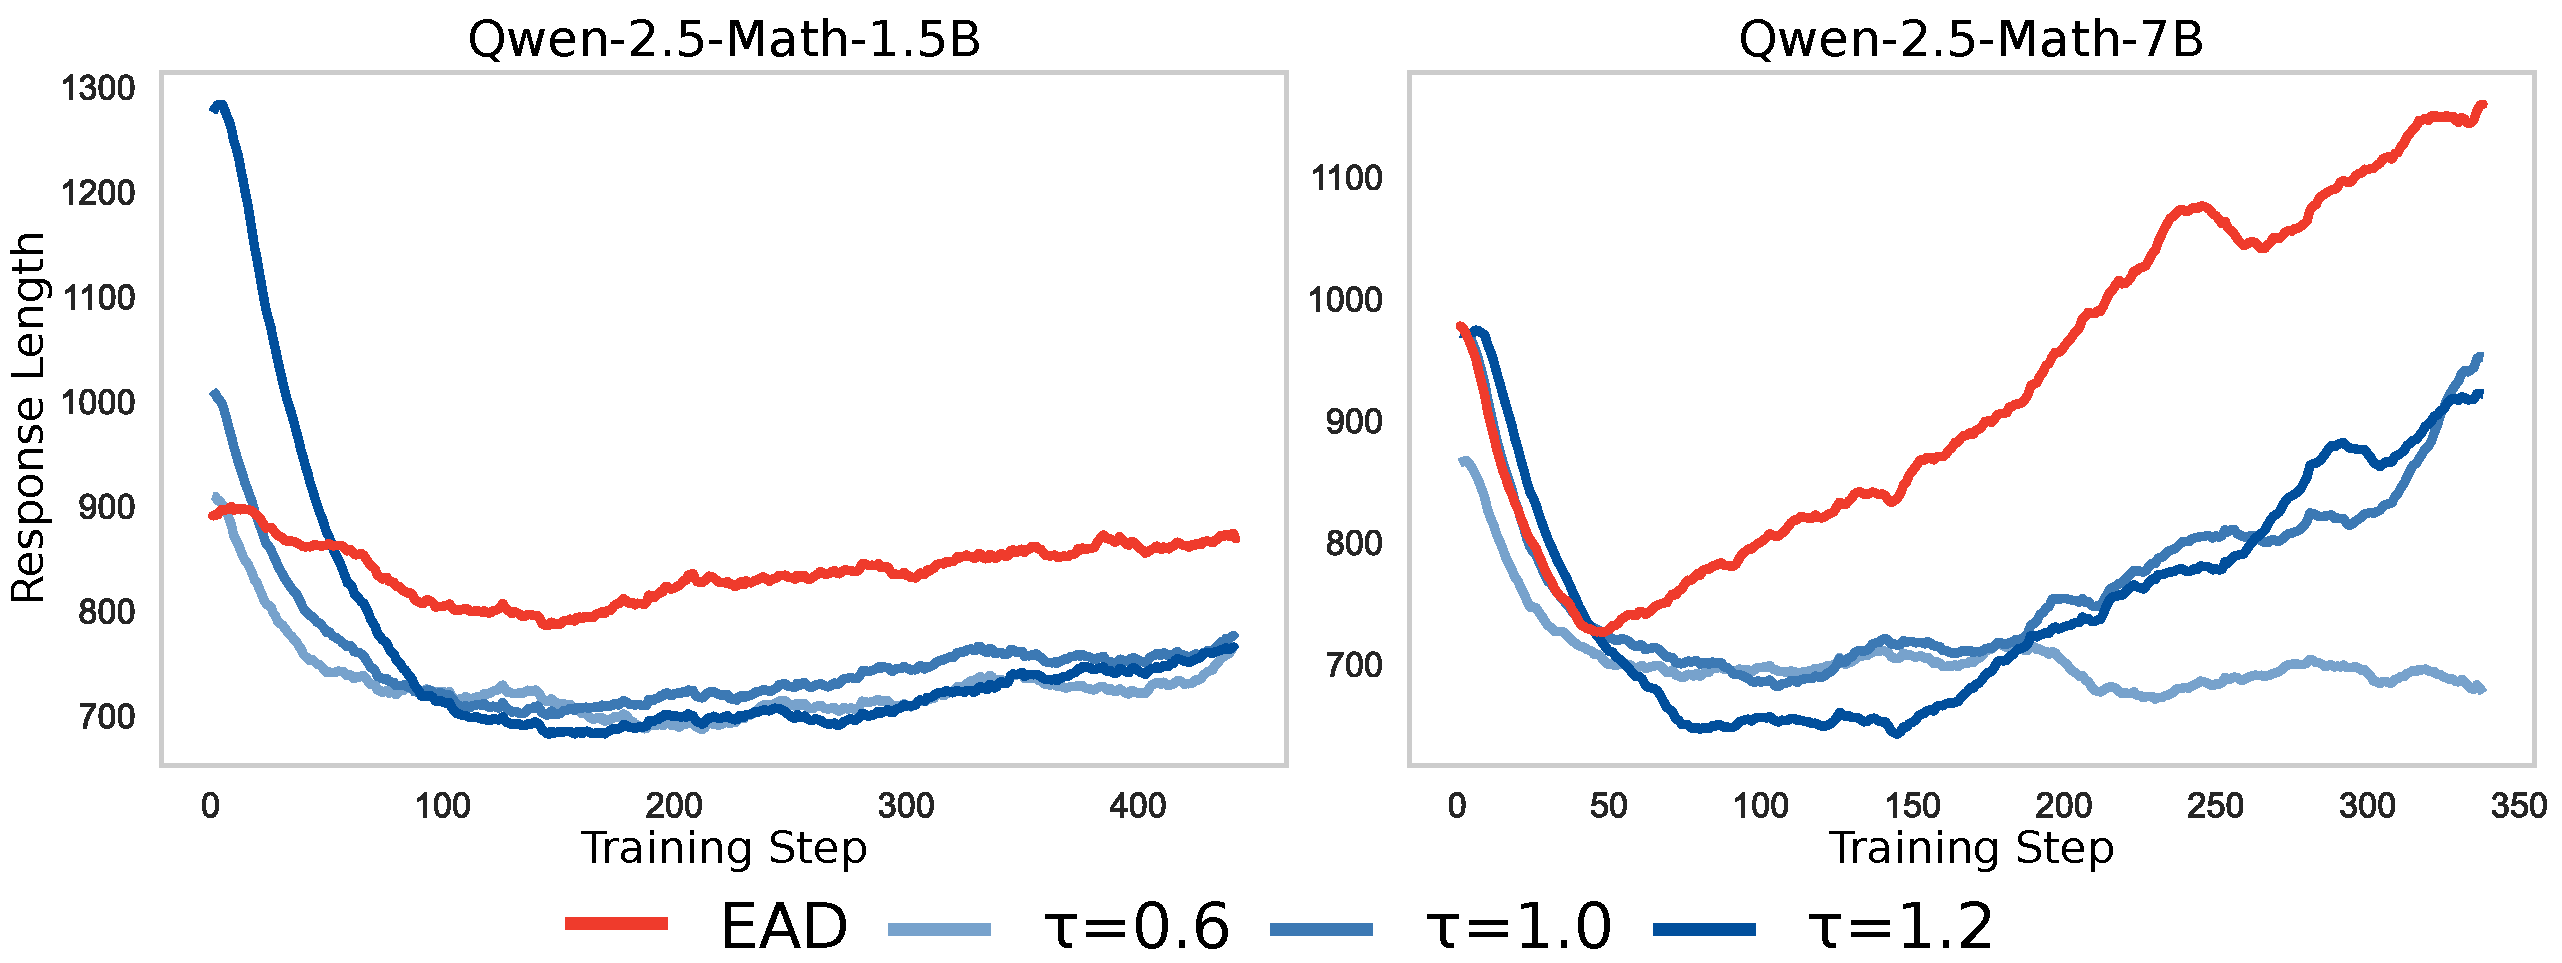
\includegraphics[width=\linewidth]{iclr2026/figures/response_length/response-length.pdf}
    % \begin{subfigure}[t]{0.49\textwidth}
    % \centering
    % 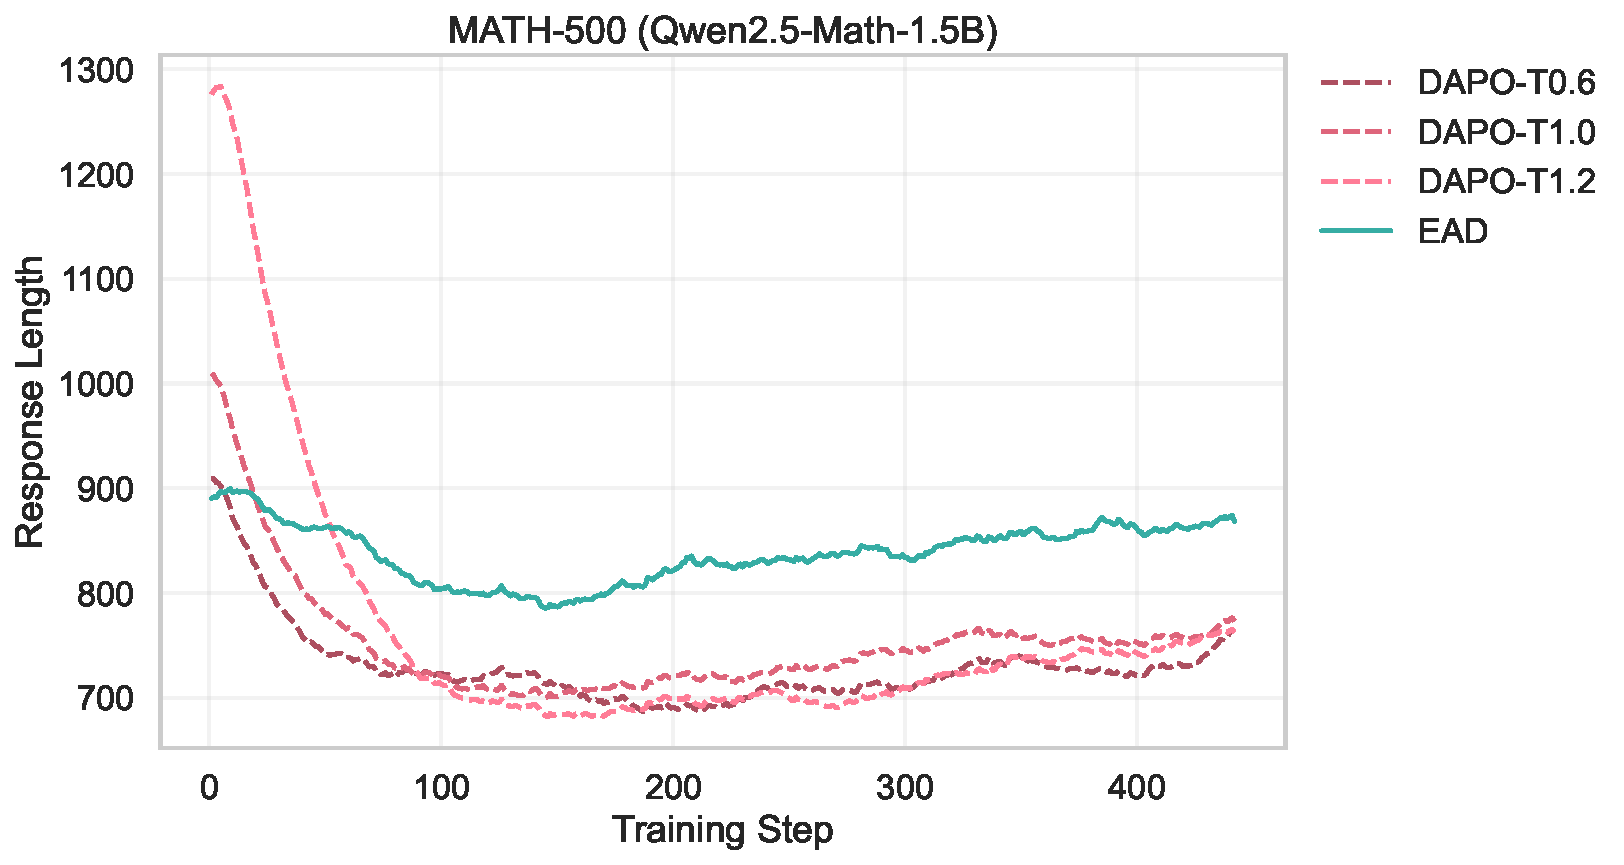
\includegraphics[width=\linewidth]{iclr2026/figures/response_length/response_length_Qwen2.5-Math-1.5B.pdf}
    % \end{subfigure}
    %     \begin{subfigure}[t]{0.49\textwidth}
    % \centering
    % 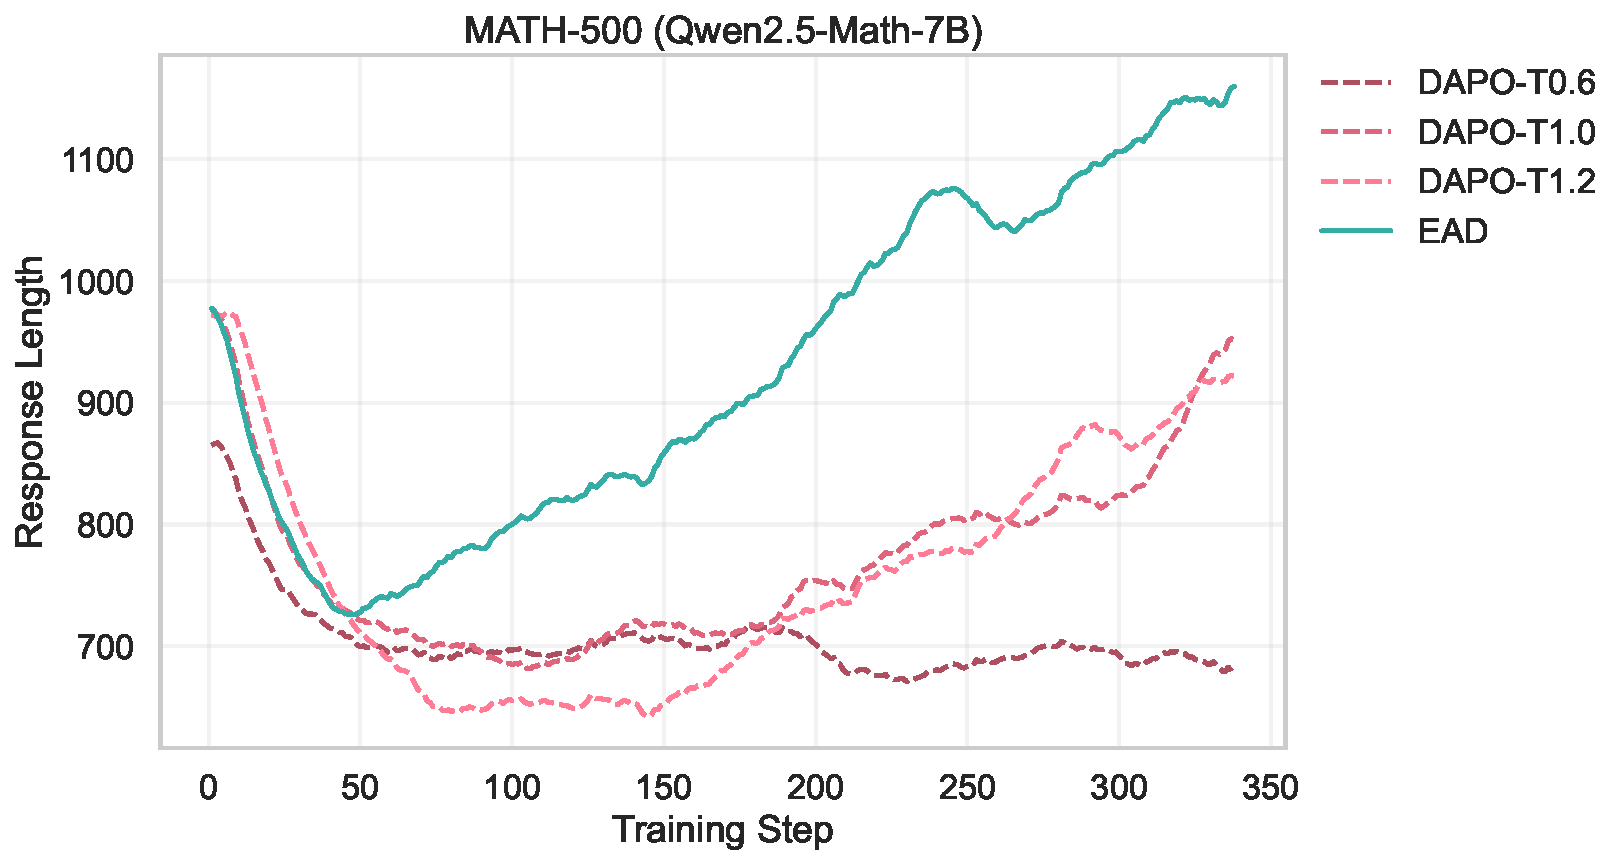
\includegraphics[width=\linewidth]{iclr2026/figures/response_length/response_length_Qwen2.5-Math-7B.pdf}
    % \end{subfigure}
\caption{Compared with normal temperature sampling, EAD can naturally incentivize the model to generate longer reasoning chains. }
\label{fig: response_length}
\end{figure}


% \section{Variance Analysis of Importance Sampling with Tempered Distributions}
% \label{app:variance_analysis_low_temp_is}
% In this section, we provide a formal analysis of the variance of an importance sampling (IS) estimator when the proposal distribution is a lower-temperature softmax transformation of the target distribution's logits. We prove that this configuration, where the proposal is less exploratory than the target, can lead to unbounded variance, making the estimator unreliable.

% \subsection{Formalism}

% Let the target distribution, $p$, and the proposal distribution, $q$, be defined by softmax functions over a set of logits $\mathbf{h} = \{h_1, h_2, \ldots, h_K\}$. The distributions are parameterized by temperatures $\tau_p$ and $\tau_q$, respectively. We use $Y$ to denote the random variable.

% The probability of selecting outcome $k$ under the target distribution $p$ is:
% \[
% p(k):=p(Y=k ;~\mathbf{h}) = \frac{\exp(h_k / \tau_p)}{\sum_{j=1}^{K} \exp(h_j / \tau_p)}.
% \]

% Similarly, the probability under the proposal distribution $q$ is:
% \[
%  q(k):=q(Y=k ;~\mathbf{h}) = \frac{\exp(h_k / \tau_q)}{\sum_{j=1}^{K} \exp(h_j / \tau_q)}.
% \]

% We consider the case where the proposal distribution is ``sharper'' or less exploratory than the target distribution, which corresponds to a lower temperature:
% \begin{equation}
%     0 < \tau_q < \tau_p
% \end{equation}

% The importance weight for an outcome $k$ is given by the ratio $w_k = {p(k)}/q(k)$. The goal of IS is to estimate the expectation of an objective $f(y)$ under $p$ by sampling from $q$: 
% \[
% \mathbb{E}_{Y\sim p}[f(Y)] = \mathbb{E}_{Y\sim q}[w_Y f(Y)].
% \]

% \subsection{Analysis of Estimator Variance}

% The variance of the IS estimator is primarily determined by the variance of the importance weights themselves. The variance of the weights under the proposal distribution $q$ is:
% \begin{equation}
%     \text{Var}_q(w) = \mathbb{E}_q[w^2] - \left(\mathbb{E}_q[w]\right)^2
% \end{equation}

% It is a standard result that $\mathbb{E}_q[w] = \sum_k q(k) \frac{p(k)}{q(k)} = \sum_k p(k) = 1$. The variance thus simplifies to:
% \begin{equation}
%     \text{Var}_q(w) = \mathbb{E}_q[w^2] - 1 = \left( \sum_{k=1}^{K} q(k) w_k^2 \right) - 1 = \left( \sum_{k=1}^{K} \frac{p(k)^2}{q(k)} \right) - 1
% \end{equation}

% For the variance to be finite, the term $\sum_{k} \frac{p(k)^2}{q(k)}$ must converge. Let's analyze the ratio $\frac{p(k)^2}{q(k)}$ by examining the weight $w_k$:
% \begin{align}
%     w_k &= \frac{p(k)}{q(k)} = \frac{\exp(h_k / \tau_p) / Z_p}{\exp(h_k / \tau_q) / Z_q} \\
%         &= \frac{Z_q}{Z_p} \exp\left(h_k \left(\frac{1}{\tau_p} - \frac{1}{\tau_q}\right)\right)
%     \label{eq:weight_expression}
% \end{align}
% where $Z_p$ and $Z_q$ are the partition functions (denominators) for their respective distributions.

% Our core assumption is that $\tau_q < \tau_p$. This implies that $\frac{1}{\tau_q} > \frac{1}{\tau_p}$, and therefore the term in the exponent of Equation~\ref{eq:weight_expression} is negative:
% \begin{equation}
%     \frac{1}{\tau_p} - \frac{1}{\tau_q} < 0
% \end{equation}

% This has a critical consequence: for outcomes $k$ with very low logits (i.e., $h_k \to -\infty$), the term $\exp(h_k (\frac{1}{\tau_p} - \frac{1}{\tau_q}))$ grows exponentially large. The low-temperature proposal distribution $q$ assigns extremely small probability to these tail-end events, far smaller than the probability assigned by the higher-temperature target distribution $p$.

% When a sample $k$ from this tail is drawn from $q$ (a rare event), its corresponding importance weight $w_k$ will be enormous. The presence of these potentially unbounded weights causes the sum $\sum_{k} \frac{p(k)^2}{q(k)}$ to diverge, leading to infinite variance.

% \paragraph{Summary and Implications} Using a lower-temperature proposal distribution ($q$) to estimate expectations over a higher-temperature target ($p$) is perilous. The proposal distribution under-samples the tails of the target distribution. On the rare occasions that a sample is drawn from these tails, the squared importance weight term $\frac{p(k)^2}{q(k)}$ can be so large that it dominates the variance calculation, often rendering it infinite.

% In the context of RL, this means that using a near-deterministic or low-entropy policy as a behavioral policy to evaluate a more stochastic target policy can lead to extremely unstable gradient estimates. This justifies the common practice of ensuring that the behavioral policy is sufficiently exploratory (i.e., has higher or equal entropy/temperature) to guarantee bounded variance and stable learning.

% \section{Usage of Large Language Models}
% In this work, besides running LLMs in experiments, we use LLMs for the following purposes:
% \begin{enumerate}
%     \item Aid or Polish Writing (Gemini 2.5 Pro, ChatGPT 4/5)
%     \item Literature Retrieval and Discovery (e.g., finding related work) (Gemini 2.5 Pro Deep Research, ChatGPT Deep Research)
%     \item Assisting Code Writing and Debugging (Claude 3.5 Sonnet)
% \end{enumerate}
% We fully understand the responsibility of using LLMs in academic research. We carefully monitor any potential problems, such as plagiarism or scientific misconduct (e.g., fabrication of facts) when using LLMs. We make sure these problems do not occur in the paper. 